\section*{Risk Evaluation}
\addcontentsline{toc}{section}{Risk Evaluation}

After having assessed the impact and likelihood scores of the threats, a risk table was adopted. 

We believe that the chosen risk table is suitable for our study since, as stated before, we want to ensure a reasonable level of security with a reasonable budget. This is because this system needs to be operational only for a limited time.

In conclusion, we found that the table in figure\ref{fig:riskTable} represents an balanced solution. 

\begin{figure}[]
    \centering
    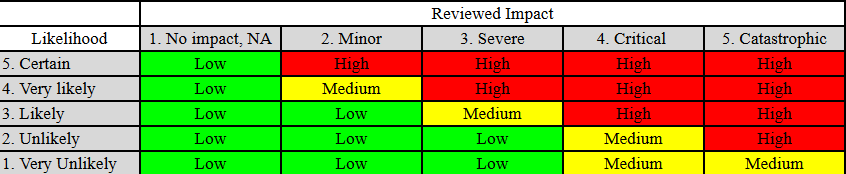
\includegraphics[keepaspectratio,width=1\textwidth]{03-risk-analysis/004-RE/img/riskTable.png}
    \caption{Risk table}
    \label{fig:riskTable}
\end{figure}

Having fixed a risk table, we proceeded to evaluate the risk level of the threats, which resulted in a high number of severe threats. The main threats that need mitigation are the ones tied to the most important assets, some of those being

\begin{itemize}
    \item \texttt{unauthorized wired connection} for the private network
    \item \texttt{hyperjacking} for the VDI
    \item \texttt{theft of equipment} for the server rooms and the secure storage of the GSBs
    \item \texttt{router crash} for the private network
    \item \texttt{phishing campaigns} for the input officials and the GSB/CSB personnel
\end{itemize}

\begin{figure}[]
    \centering
    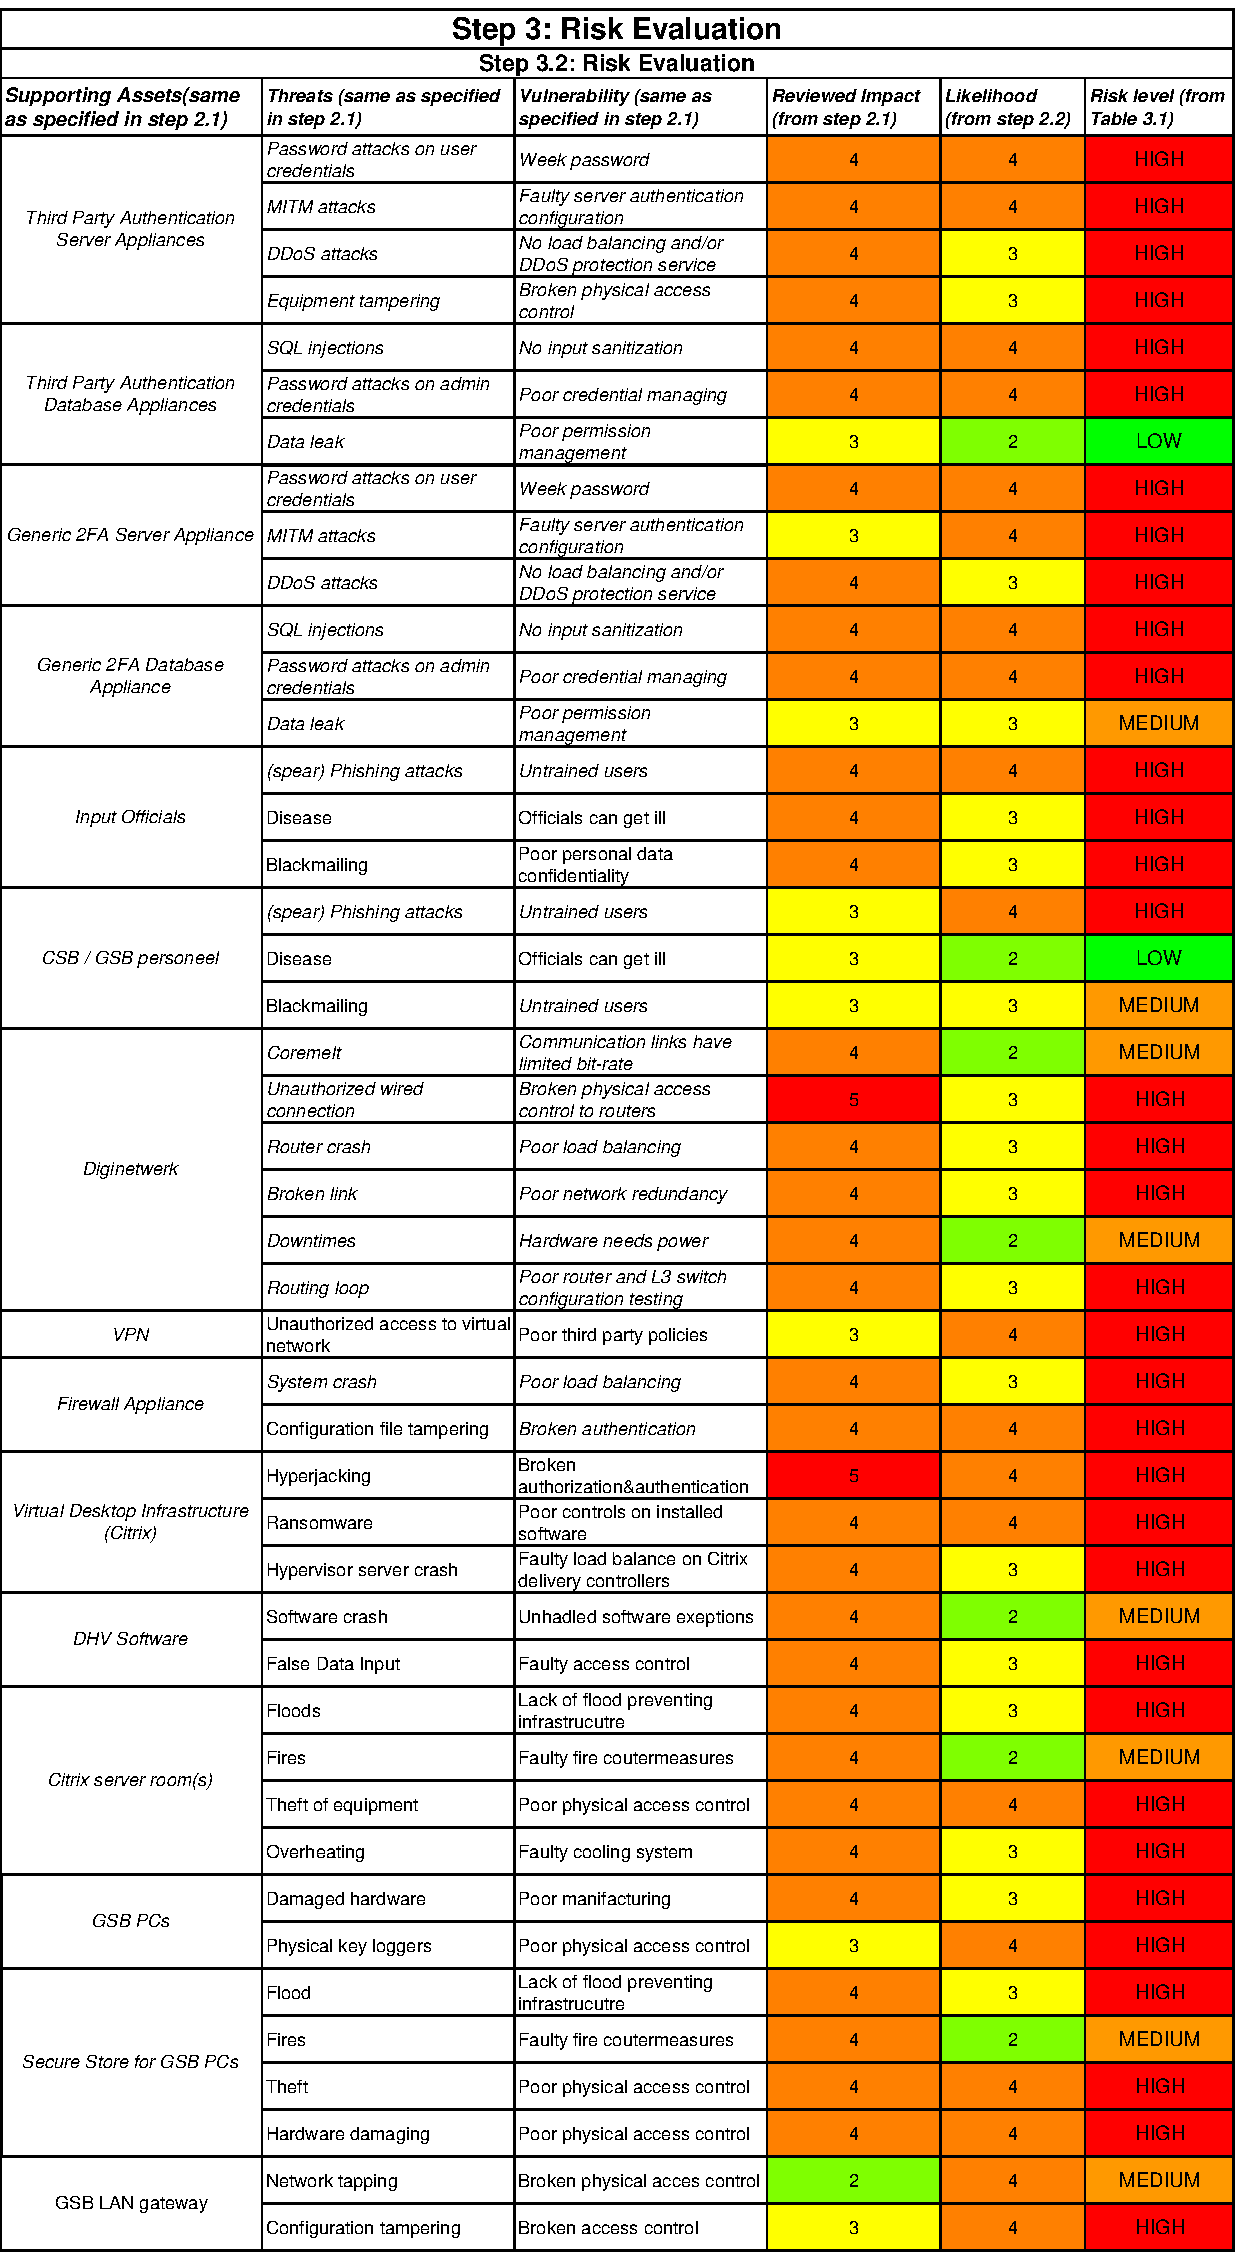
\includegraphics[keepaspectratio,width=0.8\textwidth]{03-risk-analysis/004-RE/img/riskEval.pdf}
    \caption{Risk evaluation table}
    \label{fig:riskEval}
\end{figure}